\chapter{Challenges for Posing with Line of Action}\label{chap:issues}
The line of action, both on paper and used for 3D animation, is an effective technique for the expressive posing of a character. A few main problems with the line of action arise when multiple characters interact.

\section{Maintaining Contact}
\subsection{Ground Contact}
Maintaining contact is already an issue with one character, exacerbated when more than one character is involved. Contacts for one character are constraints between the character's body parts and itself or other objects in the scene, like the floor, for instance. It would not normally be desirable to have a character's foot go through the floor; usually keeping it level with the floor is a necessary constraint.

\begin{figure}[!h]
\centering
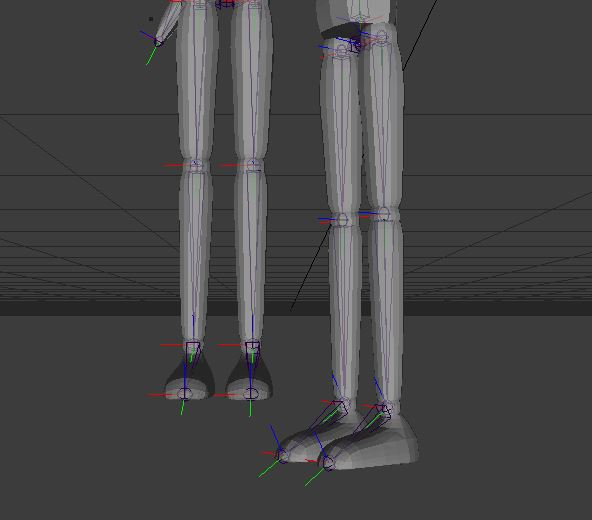
\includegraphics[scale=0.5]{img/constraint}
\caption{It's hard to tell where the floor is if every LOA moves a character closer to the target line.}
\end{figure}


\subsection{Contact Between Characters}
Now when other characters are introduced to the scene, there are even more options for potential contacts between body parts of one character and body parts of another. In our case, we only have two characters, but this research could be further generalized to a larger number of characters.

Say we want two dancers to hold each other while spinning. In one frame, it may be simple to get the characters into this specific pose without colliding with each other and touching at just the right locations. When the next keyframe is drawn, the characters may move apart from each other. In a complex dancing scene, there may be many contacts at different times changing from pose to pose, or staying constant from pose to pose. Both situations are challenging for the line of action to handle.

\begin{figure}[!h]
\centering
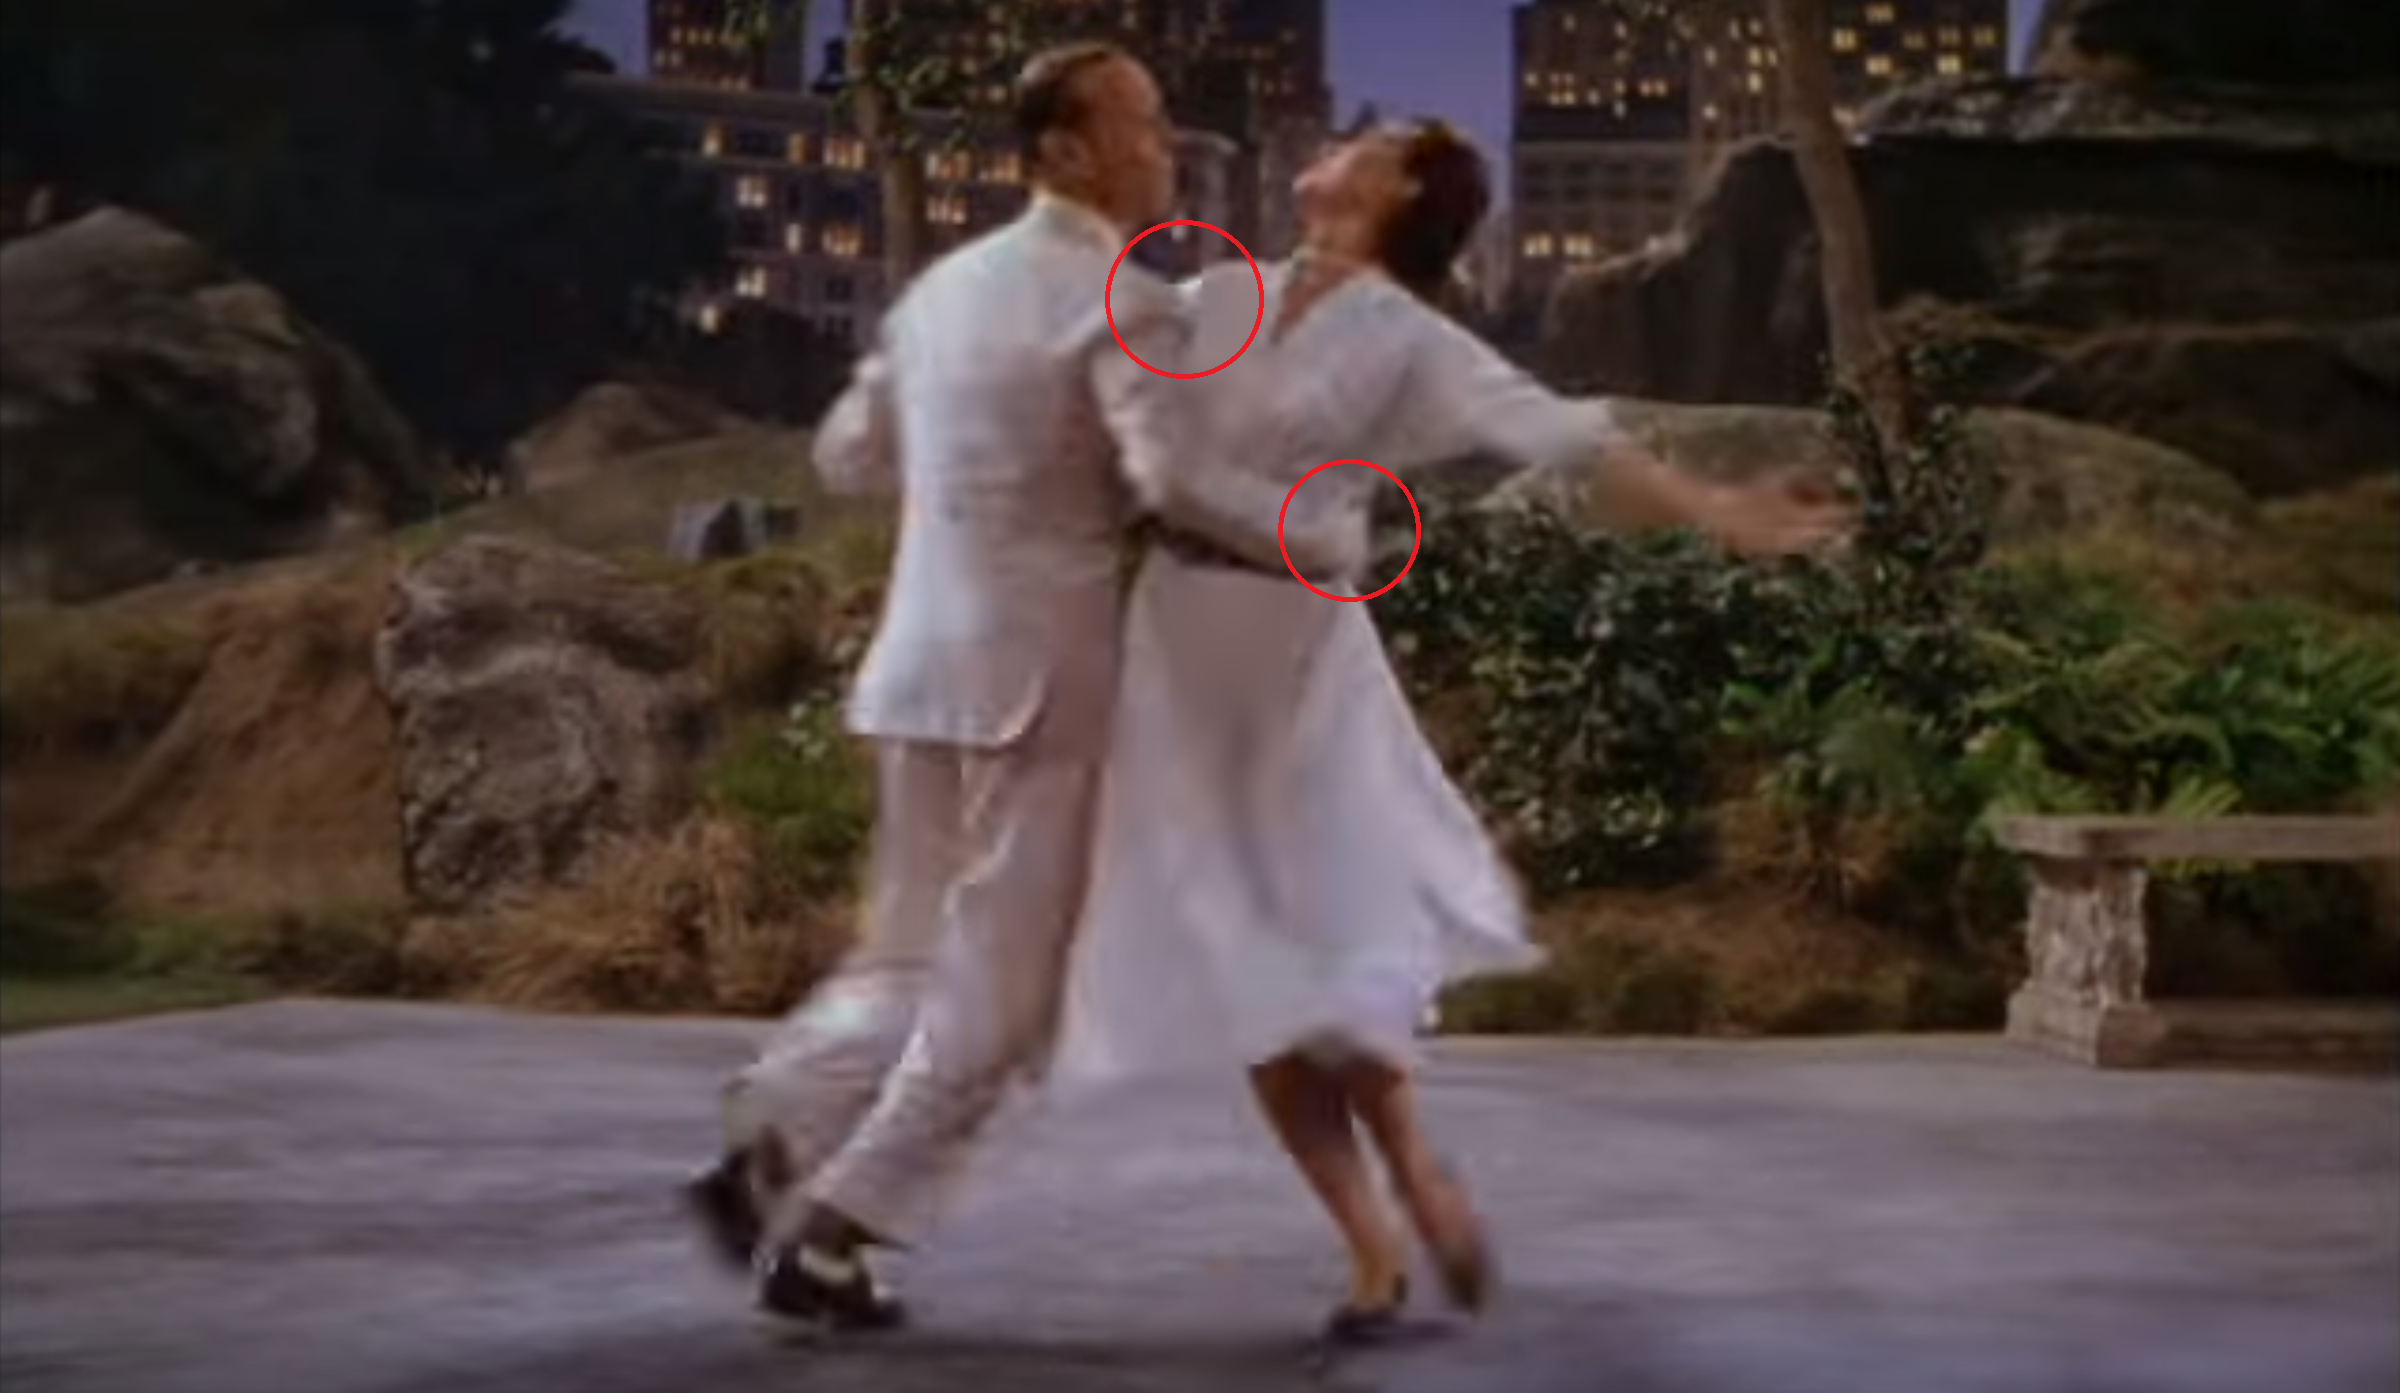
\includegraphics[scale=0.5]{img/contact}
\caption{There is clear contact between their shoulders and his hand on her hip. There are also contacts occluded in this view.}
\end{figure}

\section{Twisting}
Twisting of a 3D character is an inherently 3D problem, while LOAs are 2D lines. When a user draws a selection or posing line, the viewing plane constraint makes sure it is drawn on an invisible plane perpendicular to the camera normal. 

\begin{figure}[!h]
\centering
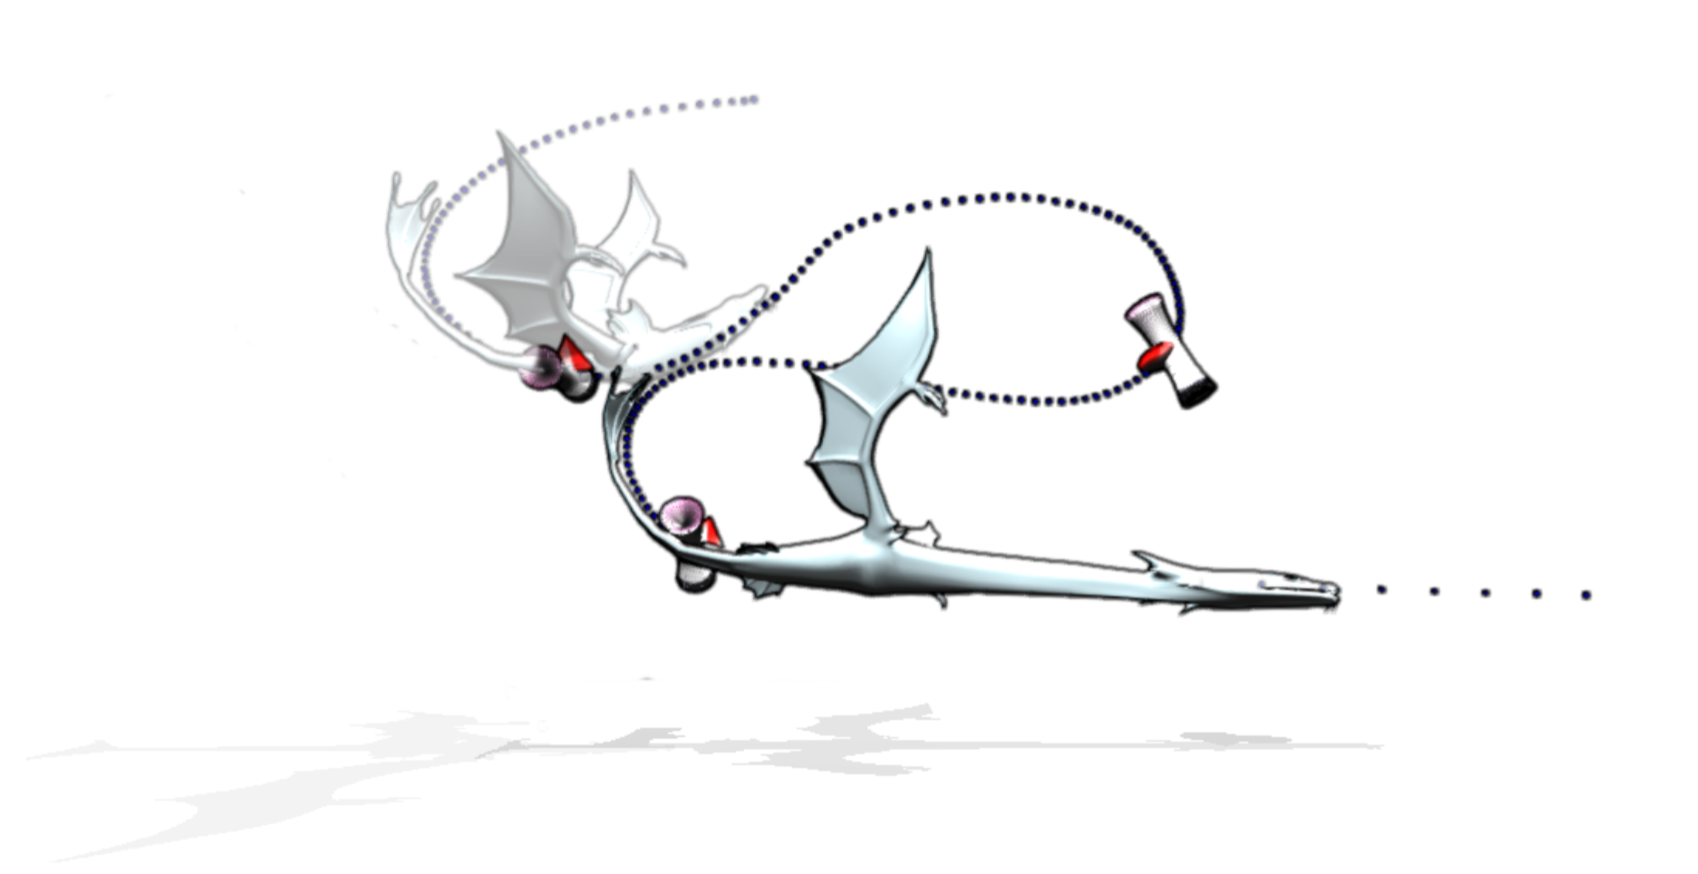
\includegraphics[scale=0.5]{img/twisting}
\caption{The dragon in \citep{guay2015space} spins around the space-time curve at specified coordinates.}
\end{figure}

The twisting in \citep{guay2015space} covers twisting within a character's body, for instance the shoulders turning while the hips stay constant. It also handles twisting around an axis for simpler characters at marked places on the space-time curve. This is not exactly the twisting seen in many dances. Twisting in dance is usually around an axis planted at the position where the character's foot makes contact with the floor.


\begin{figure}[!h]
\centering
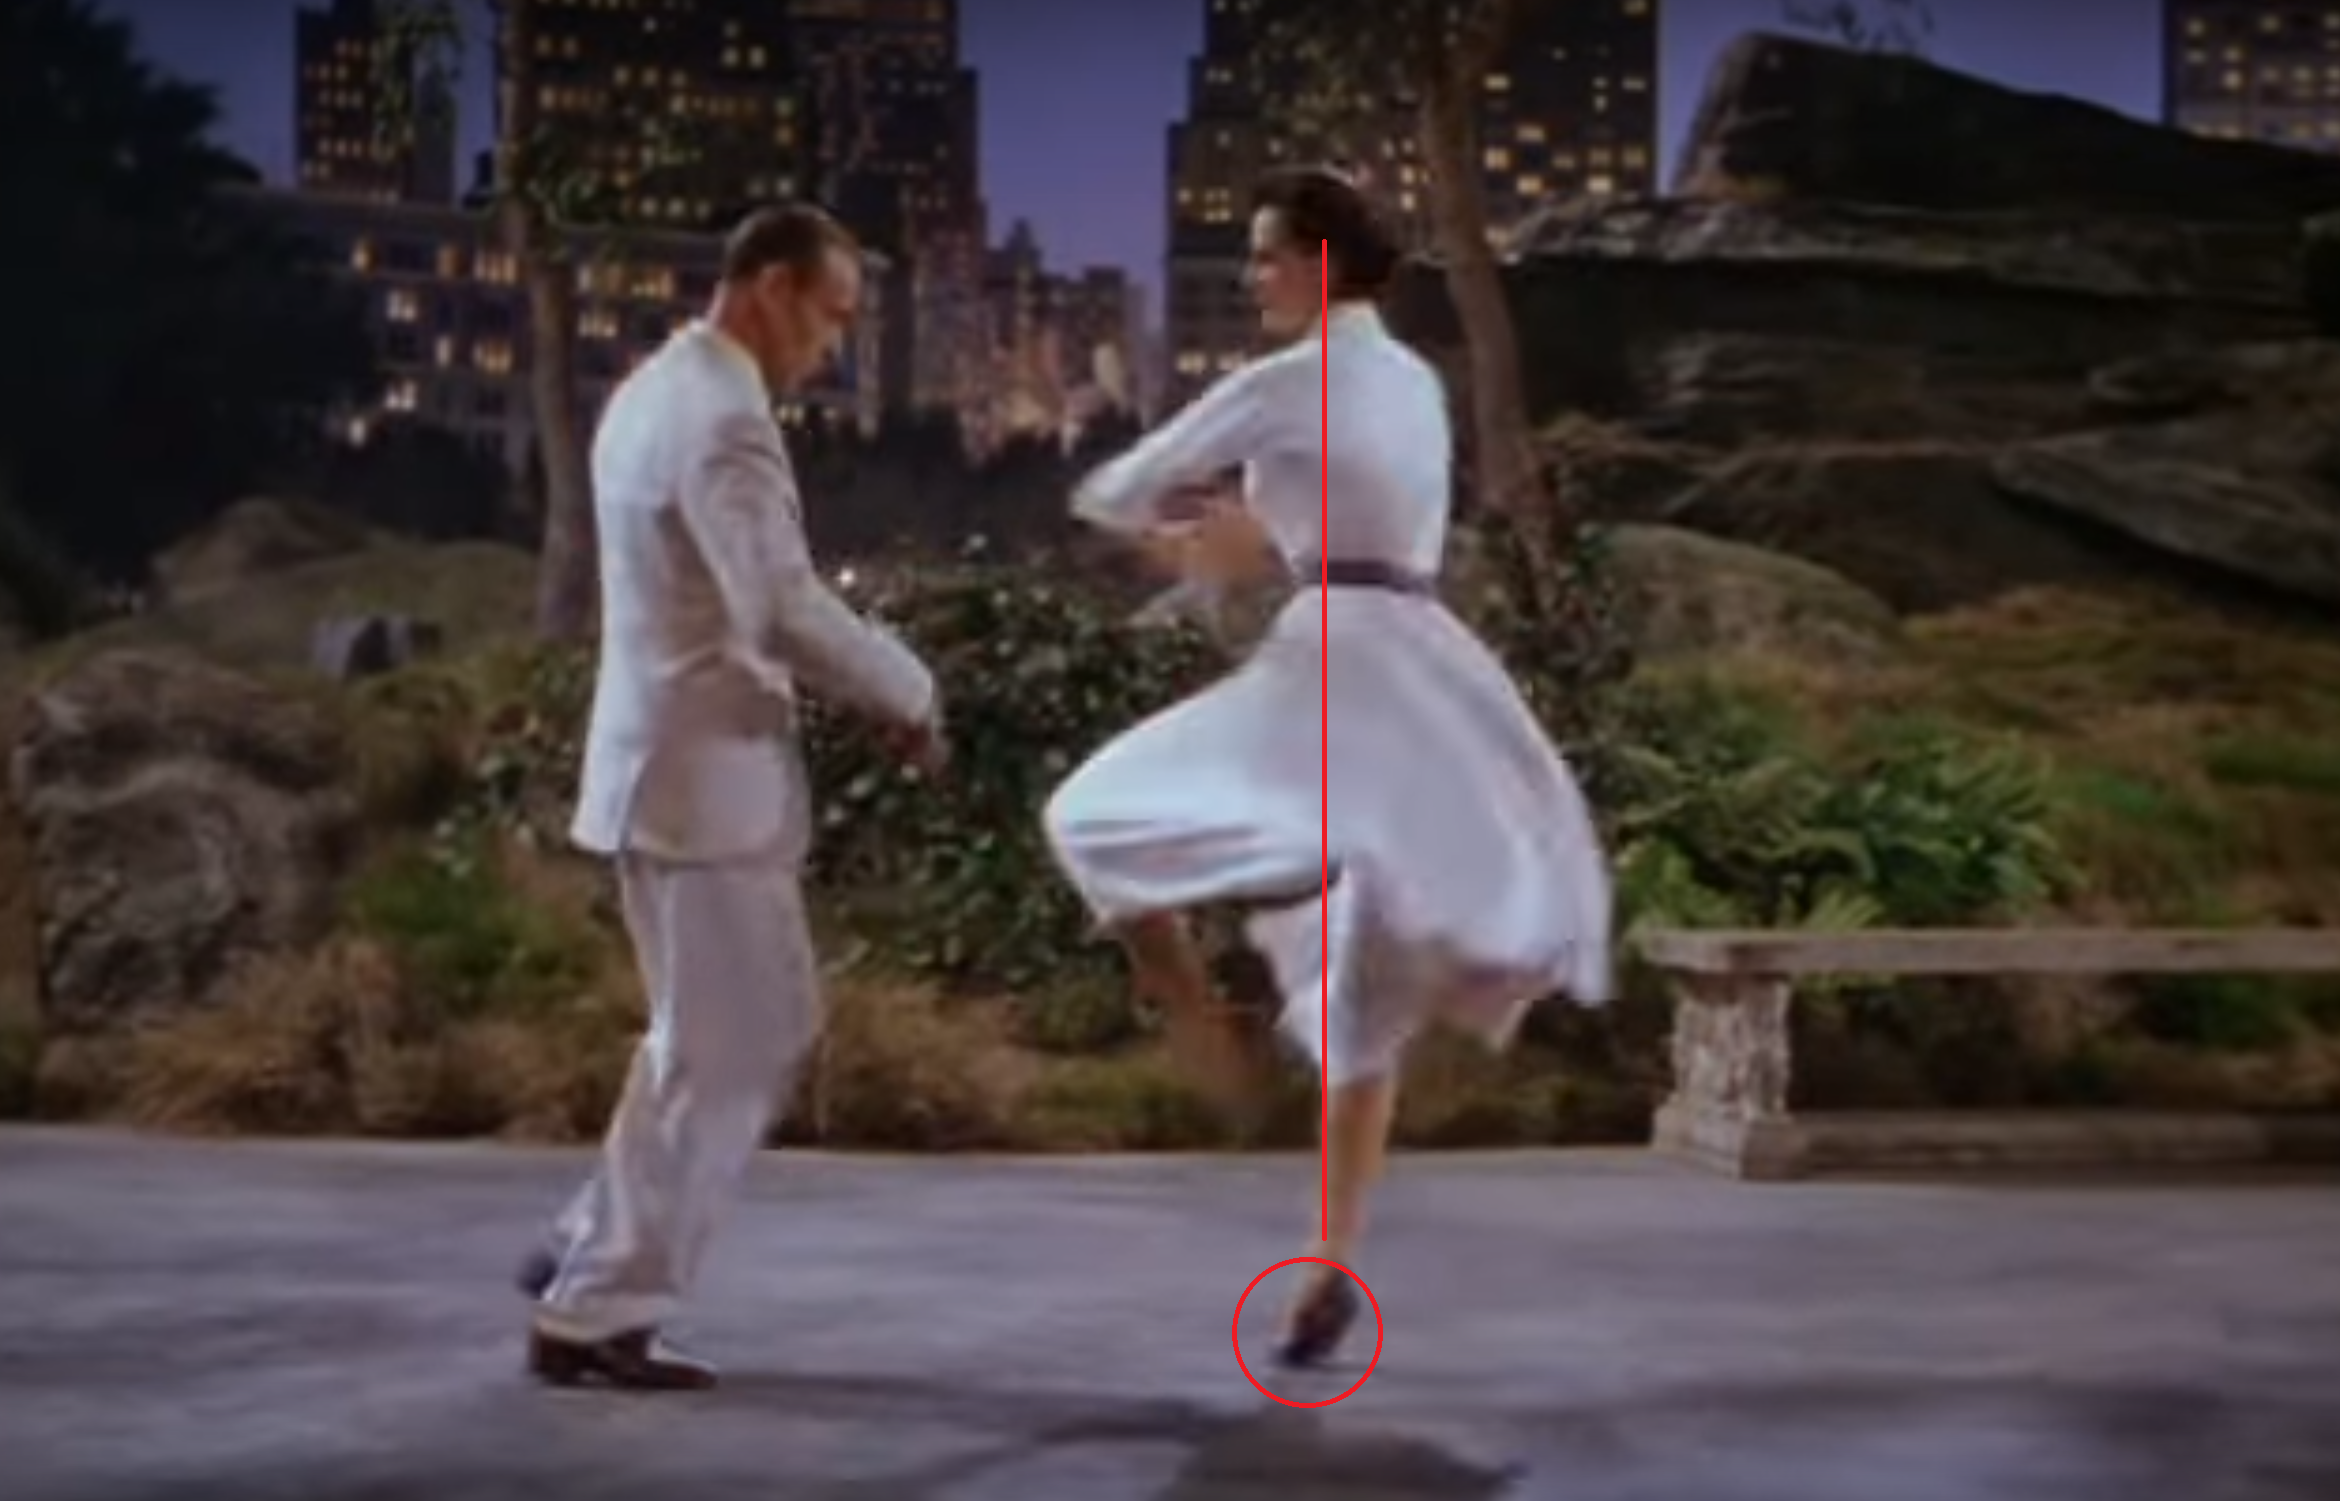
\includegraphics[scale=0.5]{img/twistinghuman}
\caption{The woman spins around her own axis maintaining contact with the ground.}
\end{figure}

%\section{Parallelism and Symmetry}

\section{Collisions}
\subsection{Self-Collisions}
\begin{figure}[h!]
	\centering
        \begin{subfigure}[b!]{0.45\textwidth}
        	\centering
                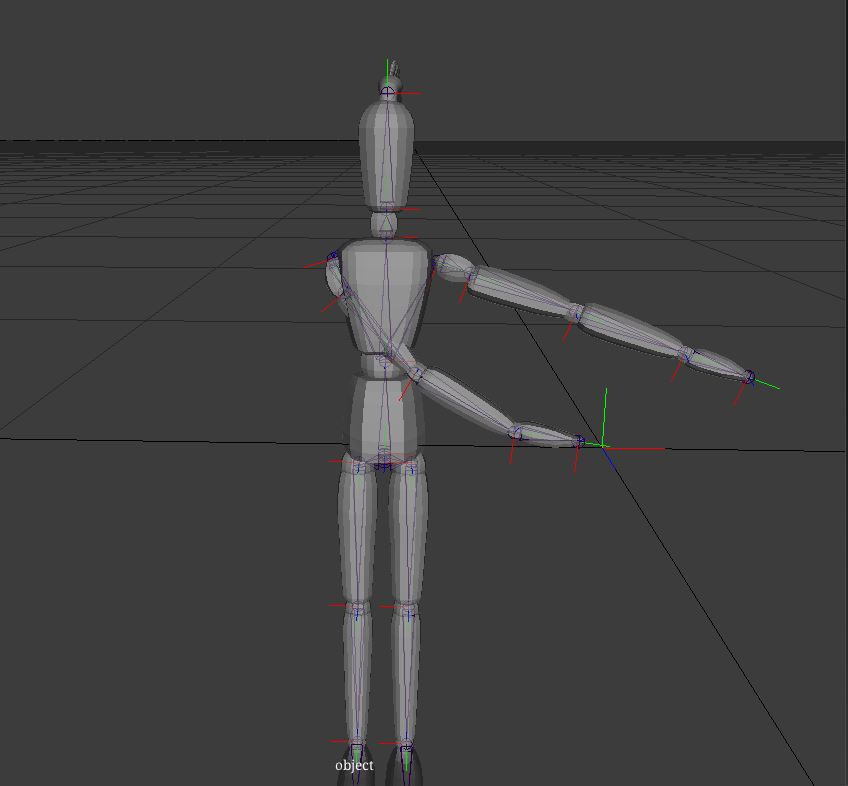
\includegraphics[width=\linewidth]{img/selfintersection}
                \label{fig:self}
                \caption{A self intersection where a character's arm goes through her body.}
        \end{subfigure}
        \quad
        \begin{subfigure}[b!]{0.45\textwidth}
        	\centering
                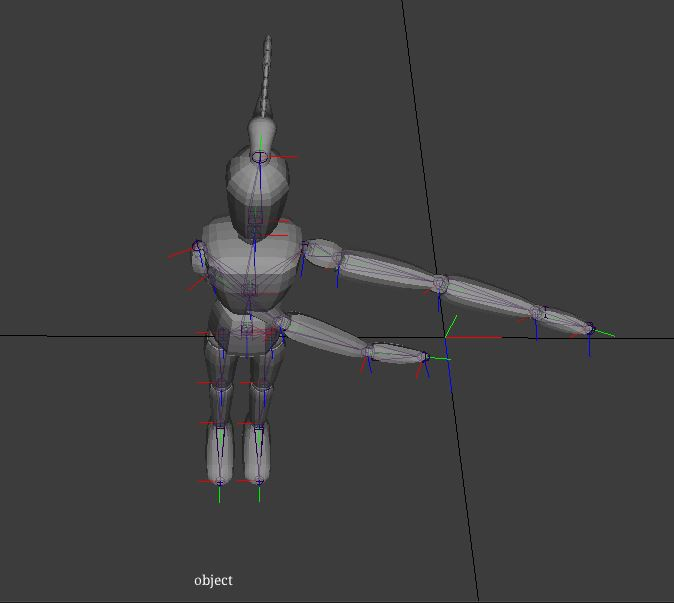
\includegraphics[width=\linewidth]{img/selfintersection1}
                \label{fig:self1}
                \caption{Another view of the self intersection.}
        \end{subfigure}%
        \caption{An example of a self-collision.}
	\label{fig:selfcollisions}
\end{figure}

Self collisions are when a part of the character's body collides with another part of its own body. The line of action technique does not do any constraint checking or collision detection, so unrealistic poses are possible. 

\subsection{Collisions Between Characters}
As the name implies, collisions between characters involve characters' body parts go through each other. Properly handling contact may solve some cases of collision.

\begin{figure}[]
	\centering
        \begin{subfigure}[b!]{0.45\textwidth}
        	\centering
                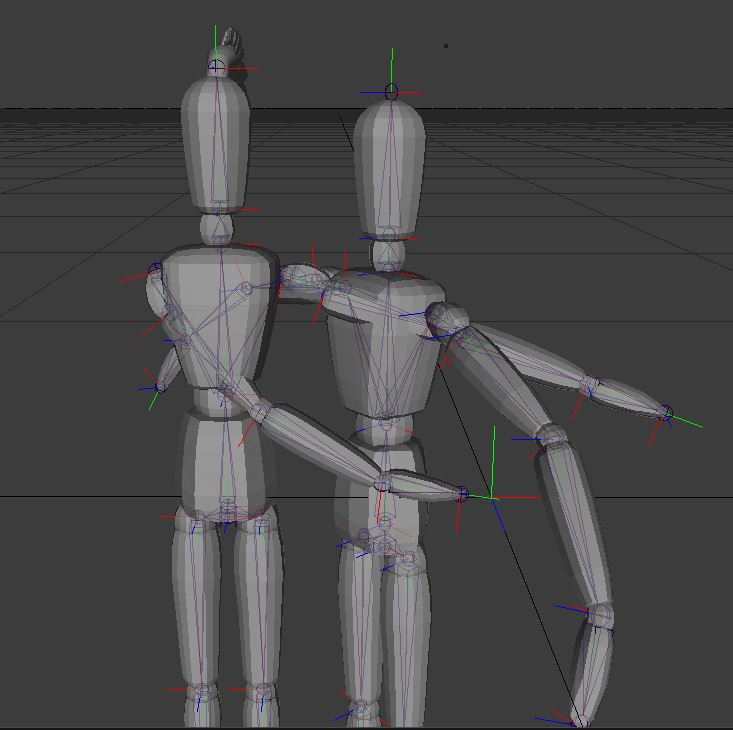
\includegraphics[width=\linewidth]{img/intersection}
                \label{fig:self}
                \caption{Two characters collide.}
        \end{subfigure}
        \quad
        \begin{subfigure}[b!]{0.45\textwidth}
        	\centering
                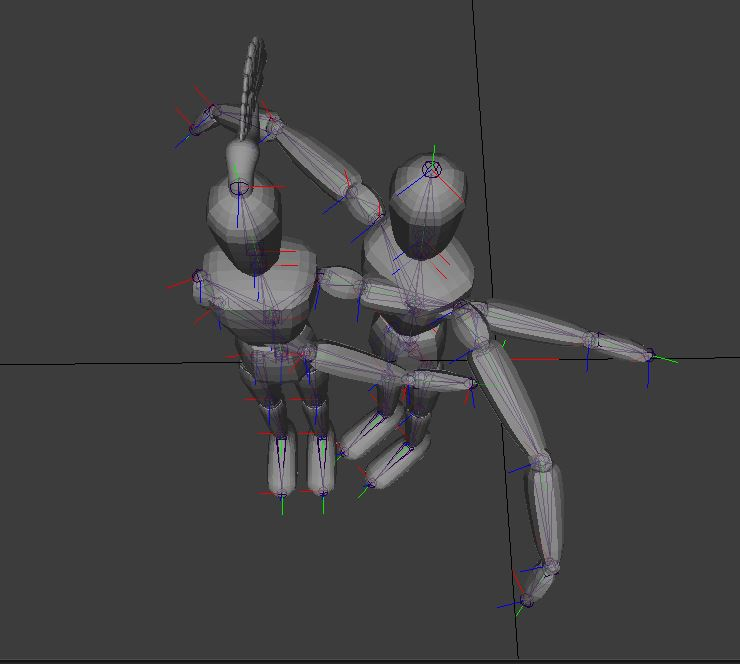
\includegraphics[width=\linewidth]{img/intersection1}
                \label{fig:self1}
                \caption{In this intersection, one character's arm goes through another's body.}
        \end{subfigure}%
        \caption{An example of a collision.}
	\label{fig:selfcollisions}
\end{figure}